Um conversor A/D tem como finalidade transformar uma grandeza física analógica em um dado digital, em um processo chamado de quantização. Já a conversão oposta, de digital para analógico, é realizada pelos conversores D/A. Um exemplo prático desse tipo de conversor são os termômetros digitais e os conversores de sinal de TV. Nesse caso, a temperatura e o sinal da TV, inicialmente grandezas analógicas, são convertidas em formato digital para que o sistema consiga processá-las e apresentá-las. O funcionamento básico desses conversores podem ser representados pelo diagrama de blocos na figura \ref{fig:diagrama-conversor}.

\begin{figure}
    \centering
    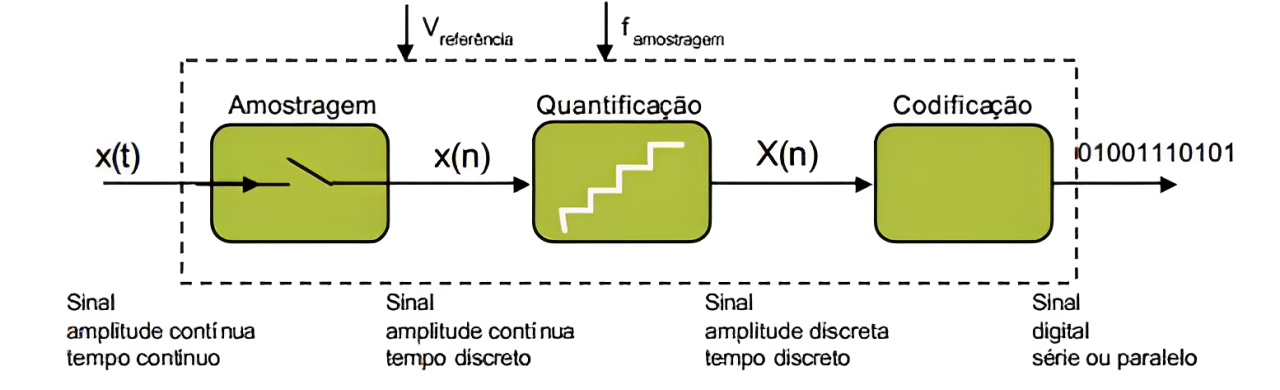
\includegraphics[width=1\linewidth]{conversorAD.png}
    \caption{Diagrama de blocos de conversor A/D}
    \label{fig:diagrama-conversor}
\end{figure}

Ao longo das décadas de estudo sobre conversores A/D, diversos modelos com diferentes princípios de funcionamento foram desenvolvidos. Entre os modelos disponíveis atualmente, destaca-se o conversor A/D de rampa dupla. Esse tipo de conversor, amplamente utilizado em multímetros digitais, apresenta vantagens significativas em relação a outros modelos, como o de rampa simples. Sua implementação é mais simples e oferece maior precisão, uma vez que elimina as variações causadas por resistores e capacitores no circuito.

O conversor A/D de Rampa Dupla é composto por elementos como resistores, capacitores, amplificadores operacionais e circuitos de controle, que atuam em conjunto para realizar a conversão do sinal analógico em digital com alta precisão. Esses componentes são organizados de forma a assegurar o funcionamento adequado das etapas de integração e desintegração do sinal. A configuração básica do conversor está ilustrada na Figura ~\ref{fig:basic_dual_slope_schematic}.

\begin{figure}[H]
    \centering
    \includesvg[width=1\linewidth]{03_results/assets/dual_slop_adc_basic_schematic.svg}
    \caption{Esquemático base do conversor ADC Rampa Dupla}
    \label{fig:basic_dual_slope_schematic}
\end{figure}

\subsection{Funcionamento do ADC de Rampa Dupla e Derivação Matemática}
O conversor ADC de Rampa Dupla opera em dois períodos de integração:

\subsubsection{Primeira Integração ($T_1$)}
Durante o período $T_1$, a chave conecta o sinal de entrada $V_I$ ao integrador. O integrador acumula a área do sinal de entrada, resultando em uma tensão $V_{CO}$ ao final de $T_1$. A duração de $T_1$ é fixa e depende da frequência do clock ($f_{clock}$) e da resolução ($N$) do conversor:
$$
    T_1 = \frac{2^N}{f_{clock}},
$$

A saída do integrador ao final de $T_1$ é dada por:
$$
    V_{CO} = -\frac{1}{R \cdot C} \int_0^{T_1} V_I \, dt = -\frac{V_I \cdot T_1}{R \cdot C}.
$$


\subsubsection{Segunda Integração ($T_2$)}
Após $T_1$, a chave conecta a tensão de referência negativa $-V_R$ ao integrador. Durante esse período, o integrador descarrega completamente, resultando em $V_{CO} = 0$ no final do tempo $T_2$. A tensão do integrador durante $T_2$ é descrita por:
\begin{align} \
    V_{CO} = -\frac{1}{R \cdot C} \left(\int_{T_1}^{T_1 + T_2} (-V_R) \, dt \right) - \frac{V_I \cdot T_1}{R \cdot C} \\
    V_{CO} = \frac{V_R \cdot T_2}{R \cdot C} - \frac{V_I \cdot T_1}{R \cdot C}.
\end{align}

Quando o capacitor descarrega completamente ($V_{CO} = 0$), temos:
$$
    \frac{V_R \cdot T_2}{R \cdot C} = \frac{V_I \cdot T_1}{R \cdot C}.
$$

Simplificando:
$$
    V_I \cdot T_1 = V_R \cdot T_2 \quad \Rightarrow \quad V_I = \frac{V_R \cdot T_2}{T_1}.
$$

\subsubsection{Relacionando o Tempo $T_2$ ao Valor Digital}
Sabendo que $T_1$ é fixo e equivale a $2^N / f_{clock}$, e que o tempo $T_2$ é proporcional ao valor digital $D$ gerado pelo contador, podemos reescrever $T_2$ como:
$$
    T_2 = D \cdot T_{clock}\, \text{, onde}\, T_{clock} = 1 / f_{clock}
$$

Substituindo $T_2$ na equação de $V_I$, temos:
$$
    V_I = V_R \cdot \frac{D \cdot T_{clock}}{T_1}.
$$

Substituindo $T_1 = 2^N / f_{clock}$:
$$
    V_I = V_R \cdot \frac{D \cdot (1 / f_{clock})}{2^N / f_{clock}} = V_R \cdot \frac{D}{2^N}.
$$

Assim, o valor digital $D$ que representa o sinal de entrada $V_I$ é dado por:
$$
    D = \frac{2^N \cdot V_I}{V_R}.
$$

Graficamente, o período de integração e desintegração de um conversor AD rampa dupla é representado pela figura \ref{fig:dual_slope_integrator_graph}, onde o período $T_{1}$ é a integração, quando o circuito integrador tem como entrada a tensão $V_{in}$ a ser convertida, e o período $T_{2}$ é a desintegração, que possui como entrada a tensão $V_{ref}$ de referência, que é fixa nas definições do projeto.
\begin{figure}
    \centering
    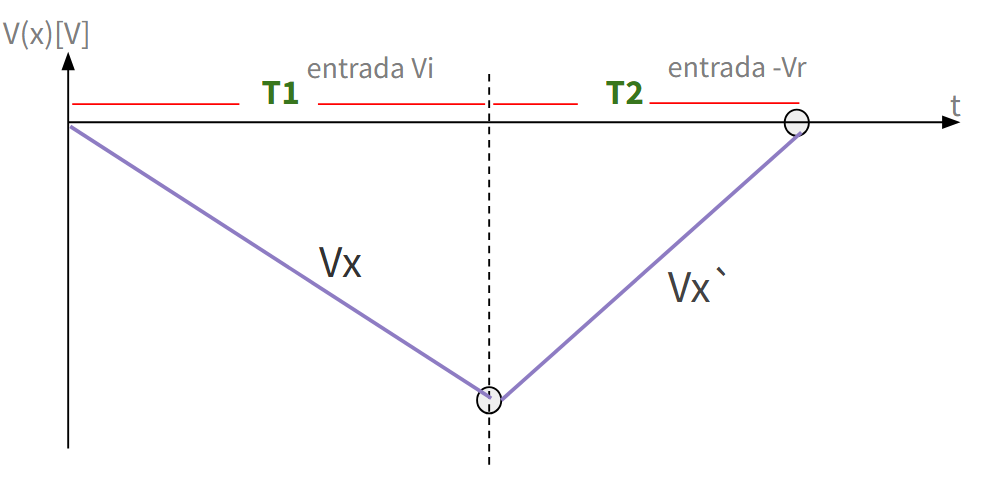
\includegraphics[width=1\linewidth]{dual_slope.png}
    \caption{Gráfico de saída do circuito integrador de um conversor rampa dupla}
    \label{fig:dual_slope_integrator_graph}
\end{figure}
